%%%%%%%%%%%%%%%%%%%%%%%%%%%%%%%%%%%%%%%%%
% University Assignment Title Page 
% LaTeX Template
% Version 1.0 (27/12/12)
%
% This template has been downloaded from:
% http://www.LaTeXTemplates.com
%
% Original author:
% WikiBooks (http://en.wikibooks.org/wiki/LaTeX/Title_Creation)
%
% License:
% CC BY-NC-SA 3.0 (http://creativecommons.org/licenses/by-nc-sa/3.0/)
% 
% Instructions for using this template:
% This title page is capable of being compiled as is. This is not useful for 
% including it in another document. To do this, you have two options: 
%
% 1) Copy/paste everything between \begin{document} and \end{document} 
% starting at \begin{titlepage} and paste this into another LaTeX file where you 
% want your title page.
% OR
% 2) Remove everything outside the \begin{titlepage} and \end{titlepage} and 
% move this file to the same directory as the LaTeX file you wish to add it to. 
% Then add \input{./title_page_1.tex} to your LaTeX file where you want your
% title page.
%
%%%%%%%%%%%%%%%%%%%%%%%%%%%%%%%%%%%%%%%%%
%\title{Title page with logo}
%----------------------------------------------------------------------------------------
%	PACKAGES AND OTHER DOCUMENT CONFIGURATIONS
%----------------------------------------------------------------------------------------

\documentclass[11pt]{article}
\usepackage[english]{babel}
\usepackage[utf8x]{inputenc}
\usepackage{amsmath}
\usepackage{graphicx}
\setlength{\marginparwidth}{2cm}
\usepackage[colorinlistoftodos]{todonotes}
\usepackage{hyperref}
\usepackage{xcolor}
\usepackage[margin=1in]{geometry}
\usepackage{tikz}
\usetikzlibrary{matrix,chains,positioning,decorations.pathreplacing,arrows}
\usetikzlibrary{trees}
\usepackage{float}
\usepackage[gen]{eurosym}
\usepackage{tasks}
\usepackage{verbatim}
\usepackage[normalem]{ulem}
\useunder{\uline}{\ul}{}
\usepackage{dirtytalk} % for quotation marks :P
\usepackage{subcaption}
\usepackage{array,ragged2e}
\usepackage{comment}
\usepackage[hybrid]{markdown}
\usepackage{algorithm} 
\usepackage{algpseudocode} 
\usepackage{tabularx}
\newcommand{\quotes}[1]{``#1''}
\usepackage{breakcites}
\usepackage{listings}
\usepackage{soul}

%%%%%CODE SNIPPETS%%%
%New colors defined below
\definecolor{codegreen}{rgb}{0,0.6,0}
\definecolor{codegray}{rgb}{0.5,0.5,0.5}
\definecolor{codepurple}{rgb}{0.58,0,0.82}
\definecolor{backcolour}{rgb}{0.95,0.95,0.92}

%Code listing style named "mystyle"
\lstdefinestyle{mystyle}{
  backgroundcolor=\color{backcolour},   commentstyle=\color{codegreen},
  keywordstyle=\color{magenta},
  numberstyle=\tiny\color{codegray},
  stringstyle=\color{codepurple},
  basicstyle=\ttfamily\footnotesize,
  breakatwhitespace=false,         
  breaklines=true,                 
  captionpos=b,                    
  keepspaces=true,                 
  numbers=left,                    
  numbersep=5pt,                  
  showspaces=false,                
  showstringspaces=false,
  showtabs=false,                  
  tabsize=2
}

%"mystyle" code listing set
\lstset{style=mystyle}
%%%%%%%%%%%%%%%%%%%%



\begin{document}

\begin{titlepage}

\newcommand{\HRule}{\rule{\linewidth}{0.5mm}} % Defines a new command for the horizontal lines, change thickness here

\center % Center everything on the page
 
%----------------------------------------------------------------------------------------
%	HEADING SECTIONS
%----------------------------------------------------------------------------------------

\textsc{\LARGE TU Delft}\\[1.2cm] % Name of your university/college
\textsc{\Large Literature Review}\\[0.5cm] % Major heading such as course name

%----------------------------------------------------------------------------------------
%	TITLE SECTION
%----------------------------------------------------------------------------------------

\HRule \\[0.4cm]
{ \huge \bfseries  Towards Off-Policy Corrective Imitation Learning}\\[0.4cm] % Title of your document
\HRule \\[1.0cm]
 

 % Towards Off-Policy Corrective Imitation Learning
%----------------------------------------------------------------------------------------
%	AUTHOR SECTION
%----------------------------------------------------------------------------------------

\begin{minipage}{0.5\textwidth}
\begin{flushleft} \large
\emph{Author:}\\
Irene \textsc{Bosque} (5051487)\\
\end{flushleft}
\end{minipage}
~
\begin{minipage}{0.4\textwidth}
\begin{flushright} \large
\emph{Supervisors:} \\
Jens \textsc{Kober}\\ %
Rodrigo \textsc{Pérez-Dattari}\\ % Supervisor's Name
Carlos \textsc{Celemin} % Supervisor's Name
\end{flushright}
\end{minipage}\\[2cm]

% If you don't want a supervisor, uncomment the two lines below and remove the section above
%\Large \emph{Author:}\\
%John \textsc{Smith}\\[3cm] % Your name

%----------------------------------------------------------------------------------------
%	DATE SECTION
%----------------------------------------------------------------------------------------

{\large February 22 2021}\\[2cm] % Date, change the \today to a set date if you want to be precise

%----------------------------------------------------------------------------------------
%	LOGO SECTION
%----------------------------------------------------------------------------------------


\includegraphics[width=6cm]{Figures/TUDelft_logo.png} % Include a department/university logo - this will require the graphicx package
 
%----------------------------------------------------------------------------------------

\vfill % Fill the rest of the page with whitespace

\end{titlepage}

\tableofcontents

\newpage
%\listoffigures
%\listoftables
%\newpage

\begin{abstract}

This document presents the preliminary literature review for the master thesis \textit{Towards Off-Policy Corrective Imitation Learning} whose objective is to improve the \textit{experience replay} implementation of the D-COACH (Deep COrrective Advice Communicated by Humans) algorithm; D-COACH is a framework in the field of Corrective Imitation Learning (CIL), where an agent is trained with feedback that a teacher provides in the form of relative corrections. Experience replay improves the sample efficiency by allowing already collected data to be used multiple times for training.  This is particularly important when training neural networks (NN) because it increases their stability helping to preserve old knowledge and thus reducing catastrophic forgetting. Furthermore, experience replay provides uncorrelated data to train the neural network which helps to generalize and to minimize overfitting. In order to use the experience replay technique, it is necessary for the algorithm to be, as it is known in reinforcement learning (RL), \textit{off-policy}. The current version of D-COACH is \textit{on-policy} and thus, the need to transform it into an off-policy version to fully leverage the benefits of experience replay. In this literature review, we first study the relevant theoretical framework, providing a general overview of reinforcement learning and what the terms on-policy and off-policy mean in that specific field. 
Then, as the main part of this review, a research in the literature is conducted for a clear definition of the terms on-policy and off-policy in imitation learning, a field where they are not as widely used as in reinforcement learning. To contribute in this aspect to the literature, two new definitions are presented and several imitation learning algorithms are classified according to these definitions. Finally, D-COACH is explained in more detail together with the proposal of how to improve the experience replay implementation by adding a new model that will predict the teacher's feedback.


% Then, I present a brief introduction to Artificial Neural Networks (ANNs) as the function approximators that are used in D-COACH including convolutional networks, autoencoders and recurrent neural networks. 
\end{abstract}
\section{Introduction}
% Introduction

Robots are increasingly present in our society; from factories to operating theatres, the demand for robots that are able to quickly adapt to changing environments does not stop growing. This necessity of fast adaptation to new situations makes hard-coding control strategies less suitable, and requires other types of flexible control approaches \cite{need-of-flexible-control-approaches}. Reinforcement learning (RL) is one of these flexible approaches where an intelligent agent tries to learn how to perform a task by maximizing a sum of rewards in a trial and error manner \cite{Sutton:1998}. RL techniques have been applied in successful cases such as \cite{Atari-RL}, \cite{alphaGO-silver-2016}, \cite{openAI-hand}, however, these examples tend to happen in simulated environments with very specific learning tasks. This fact greatly differs from real-world situations such in robotics where, in order to learn a good policy, a robot agent requires a huge amount of data, for which it will have to perform thousands of trials  \cite{reinforcement-learning-costly-Kober:2013}. This is very costly both in terms of time and the probable physical damages caused to the robot while learning \cite{TAMER-Knox-Stone:2009}. Furthermore, many real problems are easier to demonstrate than to design a reward function for applying reinforcement learning \cite{kostrikov2019imitation}. In fact, the incorporation of human knowledge in the learning process results in dramatically more efficient methods compared to autonomous learning techniques \cite{Global-overview-Attia:2018}. Imitation learning (IL) is the name of the field that leverages the knowledge of a teacher to improve the learning process. The simplest form of IL is known as behavioural cloning (BC) where an expert provides initial demonstrations of a desired task and then, an agent tries to imitate that behaviour via supervised learning.  Behavioural cloning has two main drawbacks: First, it requires demonstrations from an expert teacher which limits the possibilities of who can train the agent. And secondly, it suffers from distribution mismatch, a problem that initiates at the moment the agent deviates from the expert trajectory causing a cascade of errors that will probably make the agent fail the task.

\setlength{\parskip}{1em}

Interactive imitation learning (IIL) is a branch of imitation learning \cite{lazydagger:2021} that deals with the aforementioned issues by allowing a teacher to supervise and teach an agent \textit{during} its training. The nature of the feedback varies between frameworks; feedback in the form of evaluations (e.g., the TAMER framework \cite{TAMER-Knox-Stone:2009}) inform the agent how good or bad was the action taken. This kind of evaluative feedback is easier to implement than to define a reward function and allows a faster convergence than pure autonomous learning. However, the informativeness of this kind of evaluative feedback is still limited \cite{types-feedback-najar:2020}, and one way to improve it is to use corrections. Corrective imitation learning (CIL) is a branch of IIL that improves the informativeness of evaluative feedback, by allowing the teacher to inform the agent whether the value of a taken action should be increased or decreased \cite{Relative-corrections-Celemin:2019} and it requires less exploration compared to evaluative feedback \cite{types-feedback-najar:2020}.

\setlength{\parskip}{1em}

The goal of this master thesis is to create an extension of D-COACH (Deep COrrective Advice Communicated by Humans) \cite{ResearchAssignmentpaper}, a CIL algorithm designed for non-expert humans that uses neural networks to approximate the policy. This extension focuses on the improvement of a key component in several deep learning algorithms, experience replay \cite{Atari-RL}, a technique that uses experiences stored in a replay buffer for training. ER endows algorithms with two main advantages, these being a higher data efficiency and the ability to train with uncorrelated data \cite{Experience-Replay-zhang:2018}. These benefits are especially useful when policies are approximated with neural networks because already collected experiences can be reused multiple times and the neural network gets more robust against locally overfitting to the most recent trajectories, a phenomenon known as \textit{catastrophic forgetting}. The incorporation of ER into an algorithm requires that said algorithm is what in RL is known as off-policy \cite{Sutton:1998}. According to Sutton and Barto, off-policy learning occurs when a policy is updated with data gathered \say{off} that policy. The existing version of D-COACH is on-policy, because the policy is updated with data that depends on its most recent version. Despite being on-policy, current D-COACH uses experience replay for data-efficiency purposes. Given that the algorithm is on-policy, the size of the replay buffer has to be small, which works under the assumption that the data stored in the replay buffer is still valid for the current version of the policy, even if it was collected by an older version of itself. As the size of the replay buffer starts to increase, this assumption does not hold anymore and the training of the policy will most likely fail. If we want to have a more general framework, this restriction has to be removed and this is precisely the objective of this master thesis.






\setlength{\parskip}{1em}

This literature review is organized in the following manner: In section \ref{section:Reinforcement-Learning}, the basics of reinforcement learning are presented,a theoretical background that is necessary for later better understand imitation learning and the terms on-policy and off-policy. In section \ref{section:Imitation-Learning}, after explaining what is imitation learning, several IL algorithms are gathered and classified according to our proposed definitions of on-policy and off-policy imitation learning. Lastly, section \ref{section:Towards-off-policy-CIL} focuses on D-COACH and the proposal of how to transform it into an off-policy version to better leverage the benefits of experience replay.






\input{C_Content}
\section{Conclusions}


Sections \ref{section:Reinforcement-Learning}, \ref{section:Imitation-Learning} and \ref{section:Towards-off-policy-CIL} present the theoretical relevant  background for this master thesis. Specifically, section \ref{section:Reinforcement-Learning} introduces reinforcement learning and how it makes use of MDPs as a framework for sequential decision making problems. The review continues explaining what the terms on-policy and off-policy mean in RL with the help of SARSA and Q-learning algorithms. This section ends with the concept of experience replay, a technique  that is a critical part of this thesis. In section \ref{section:Imitation-Learning} we introduce the concept of imitation learning, a machine learning method that leverages human knowledge in the learning process being more efficient than pure autonomous learning approaches in complex real-world problems. We present the definitions found in the literature of the terms on-policy and off-policy in imitation learning together with our interpretation with which several IL algorithms are classified.
This literature review ends with section \ref{section:Towards-off-policy-CIL} where we explain in more detail the algorithm COACH and its deep version D-COACH. There, it is explained why D-COACH needs to be transformed into an off-policy algorithm to fully leverage experience replay. Finally, we present the proposal of how to carry on this transformation by introducing a new model in the D-COACH framework that will predict the human's feedback.




\newpage
\appendix

%\section{Function approximation}



%A policy, normally called $\pi$, maps observations of a learning agent to the actions it takes. 
%For simple environments a policy can be represented with a lookup table but as the state space increases, representing the policy in a tabular manner becomes infeasible. Here is where function approximation come into play. Function approximation are different techniques that estimate a function that represents the policy as a parametrized model $\pi_\theta$ where $\theta$ represents the parameters of said model. The function approximator to be learned, $\psi$, needs to represent the policy as $\pi_\theta=\psi(s;\theta)$ in a way  that $\psi: S \rightarrow A$ defines the mapping from the state space to the action space, (add reference!). One of these techniques are Artificial Neural Networks and I am going to focus on them because they are the focus of this thesis.






\section{Artificial Neural Networks}

An Artificial Neural Network or ANN is a computational model formed by a connection of artificial neurons arranged in structures called layers, \cite{ANN-graupe:2013}. Every ANN possesses three types of layers, the input layer, the hidden layer(s) and the output layer, see figure \ref{fig:ANN}.
\begin{figure}[H]
\centering
\begin{tikzpicture}[
plain/.style={
  draw=none,
  fill=none,
  },
net/.style={
  matrix of nodes,
  nodes={
    draw,
    circle,
    inner sep=10pt
    },
  nodes in empty cells,
  column sep=2cm,
  row sep=-9pt
  },
>=latex
]
\matrix[net] (mat)
{
|[plain]| \parbox{1.3cm}{\centering Input\\layer} & |[plain]| \parbox{1.3cm}{\centering Hidden\\layer} & |[plain]| \parbox{1.3cm}{\centering Output\\layer} \\
& |[plain]| \\
|[plain]| & \\
& |[plain]| \\
  |[plain]| & |[plain]| \\
& & \\
  |[plain]| & |[plain]| \\
& |[plain]| \\
  |[plain]| & \\
& |[plain]| \\    };
\foreach \ai [count=\mi ]in {2,4,...,10}
  \draw[<-] (mat-\ai-1) -- node[above] {Input \mi} +(-2cm,0);
\foreach \ai in {2,4,...,10}
{\foreach \aii in {3,6,9}
  \draw[->] (mat-\ai-1) -- (mat-\aii-2);
}
\foreach \ai in {3,6,9}
  \draw[->] (mat-\ai-2) -- (mat-6-3);
\draw[->] (mat-6-3) -- node[above] {Ouput} +(2cm,0);
\end{tikzpicture}
\caption{Diagram of an Artificial Neural Network, \cite{NN-tikz}} \label{fig:ANN}
\end{figure}





An artificial neuron, see figure \ref{fig:neuron}, is the simplest element of an ANN. Similar to a biological neuron, an artificial neuron has input connections through which it receives external stimuli, the input data $x$, \cite{ANN-graupe:2013}; With these inputs, the neuron makes a computation and generates an output value. This computation is a weighted sum of the input data where the weights $w$ are the parameters of the model that have to be adjusted in order for the model to learn. Furthermore, there is an additional input connection to the neuron, the parameter bias $b$ that also gets added to the weighted sum, $wx + b$. The final element of the artificial neuron is the activation function $f$ that takes as input the previous weighted sum and distorts it by adding non-linear deformations, $f(wx + b)$.

\begin{figure}[H]
\centering
\begin{tikzpicture}[
init/.style={
  draw,
  circle,
  inner sep=2pt,
  font=\Huge,
  join = by -latex
},
squa/.style={
  draw,
  inner sep=2pt,
  font=\Large,
  join = by -latex
},
start chain=2,node distance=13mm
]
\node[on chain=2] 
  (x2) {$x_2$};
\node[on chain=2,join=by o-latex] 
  {$w_2$};
\node[on chain=2,init] (sigma) 
  {$\displaystyle\Sigma$};
\node[on chain=2,squa,label=above:{\parbox{2cm}{\centering Activation \\ function}}]   
  {$f$};
\node[on chain=2,label=above:Output,join=by -latex] 
  {$y$};
\begin{scope}[start chain=1]
\node[on chain=1] at (0,1.5cm) 
  (x1) {$x_1$};
\node[on chain=1,join=by o-latex] 
  (w1) {$w_1$};
\end{scope}
\begin{scope}[start chain=3]
\node[on chain=3] at (0,-1.5cm) 
  (x3) {$x_3$};
\node[on chain=3,label=below:Weights,join=by o-latex] 
  (w3) {$w_3$};
\end{scope}
\node[label=above:\parbox{2cm}{\centering Bias \\ $b$}] at (sigma|-w1) (b) {};

\draw[-latex] (w1) -- (sigma);
\draw[-latex] (w3) -- (sigma);
\draw[o-latex] (b) -- (sigma);

\draw[decorate,decoration={brace,mirror}] (x1.north west) -- node[left=10pt] {Inputs} (x3.south west);
\end{tikzpicture}
\caption{Neuron diagram, \cite{NN-tikz}} \label{fig:neuron}
\end{figure}

ANNs can be classified according to multiple taxonomies, one of them refers to the direction in which the data is propagated through the layers, giving, as a result, two main groups: feedforward neural networks (FNN) and recurrent neural networks (RNN), \cite{Classification-Artificial-Neural-Networks:2017}.

\subsection{Feedforward Neural Networks (FNNs)}

A feedforward neural network (FNN) is a type of artificial neural network where information flows in only one direction from the input layer to the output layer without going through any loop.
  \vspace{1mm} \\


\subsection{Recurrent Neural Networks (RNNs)}

Opposite to feedforward neural networks, recurrent neural networks (RNNs) propagate data both forwards and backwards through the layers endowing the model with memory. RNNs are especially useful when dealing with sequential or time-dependent where some information underlays hidden, e.g., temporal information.

\vspace{5mm} 
\textbf{1. Vanilla RNN}

Vanilla RNNs are the simplest version of recurrent networks (Figure \ref{fig:rnn} shows an unrolled Vanilla RNN cell). The hidden state $h$ is a parameter whose dimension is defined by the user and it is this parameter $h$ the one that forms the recurrent connection within the cell. The hidden state at time $t$, $h_t$ is computed by adding the input data at that time, $x_t$, plus the hidden state from the previous time step $h_{t-1}$, see equation \ref{eq:vanilla_rnn}. It is precisely the fact of adding information from previous states, which makes the model able to remember.

%\begin{figure}[H]
\centering
\begin{tikzpicture}[item/.style={circle,draw,thick,align=center},
itemc/.style={item,on chain,join}]
 \begin{scope}[start chain=going right,nodes=itemc,every
 join/.style={-latex,very thick},local bounding box=chain]
 \path node (A0) {$A$} node (A1) {$A$} node (A2) {$A$} node[xshift=2em] (At)
 {$A$};
 \end{scope}
 \node[left=1em of chain,scale=2] (eq) {$=$};
 \node[left=2em of eq,item] (AL) {$A$};
 \path (AL.west) ++ (-1em,2em) coordinate (aux);
 \draw[very thick,-latex,rounded corners] (AL.east) -| ++ (1em,2em) -- (aux) 
 |- (AL.west);
 \foreach \X in {0,1,2,t} 
 {\draw[very thick,-latex] (A\X.north) -- ++ (0,2em)
 node[above,item,fill=gray!10] (h\X) {$h_\X$};
 \draw[very thick,latex-] (A\X.south) -- ++ (0,-2em)
 node[below,item,fill=gray!10] (x\X) {$x_\X$};}
 \draw[white,line width=0.8ex] (AL.north) -- ++ (0,1.9em);
 \draw[very thick,-latex] (AL.north) -- ++ (0,2em)
 node[above,item,fill=gray!10] {$h_t$};
 \draw[very thick,latex-] (AL.south) -- ++ (0,-2em)
 node[below,item,fill=gray!10] {$x_t$};
 \path (x2) -- (xt) node[midway,scale=2,font=\bfseries] {\dots};
\end{tikzpicture}
\caption{Vanilla RNN} \label{fig:rnn}
\end{figure}

\begin{figure}[H]
    \centering
    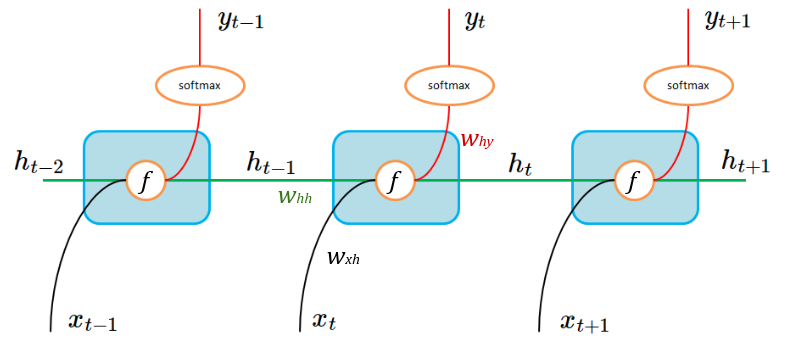
\includegraphics[width=.7\textwidth]{Figures/rnn.png}
    \caption{Vanilla Recurrent Neural Network, \cite{Vanilla-RNN-image}}
    \label{fig:rnn}
\end{figure}



\begin{equation}
h_t=tanh(W_{xh}x_t+W_{hh}h_{t−1})
\end{equation}


\begin{equation}
h_t = tanh\left(\begin{pmatrix}
W_{xh} & W_{hh}
\end{pmatrix}
\begin{pmatrix}
x_t \\
h_{t−1} \\
\end{pmatrix}\right)
\label{eq:vanilla_rnn}
\end{equation}


Vanilla RNNs suffer from a problem called vanishing/exploding gradient that makes them unable to work properly with big temporal horizons. Here is where long short-term memory (LSTM) come to play.

\vspace{5mm} 
\textbf{2. Long Short-Term Memory (LSTM)}

LSTMs are an improved version of the Vanilla RNN; They are able to learn long term dependencies by maintaining not only the hidden state $h$ but also a cell state $c$ which is the key of these networks. Furthermore, an LSTM cell includes four gates that control the flow of information to the cell state.

\subsection{Convolutional Neural Networks (CNNs)}


A convolutional neural network is a special type of ANN mostly used when the input data are images from which we want to extract information. To achieve this, filters (also called kernels) convolve on the input data producing feature maps. An example of how this convolution is done can be seen in figure \ref{fig:cnn}. The filter (blue) slides over the input image (red) and at every location, a matrix multiplication takes place giving, as a result, a feature map (green). The objective of these CNNs is to learn the filters in order to detect patterns in the input images.
\begin{figure}[H]
\centering
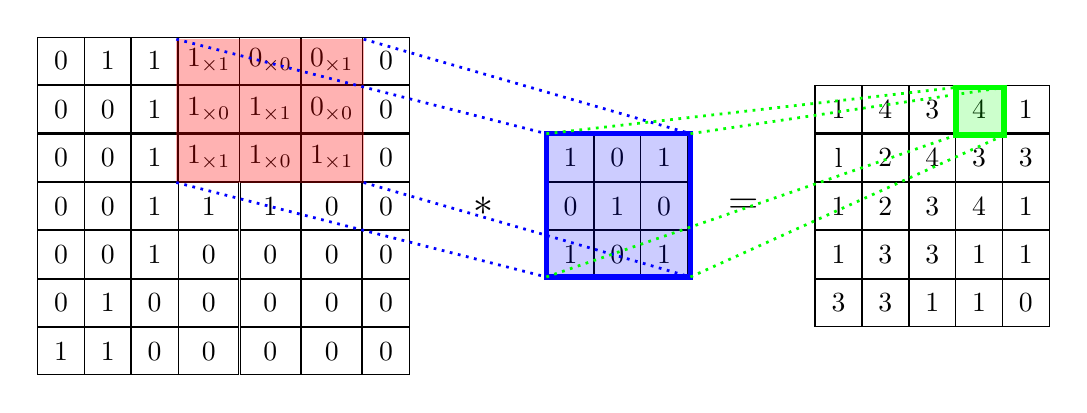
\begin{tikzpicture}[scale=1]

  \matrix [nodes=draw,column sep=-0.2mm, minimum size=6mm]
  {
    \node {0}; & \node{1}; & \node {1}; & \node{$1_{\times 1}$}; & \node{$0_{\times 0}$}; 
    & \node{$0_{\times 1}$}; & \node{0}; \\
    \node {0}; & \node{0}; & \node {1}; & \node{$1_{\times 0}$}; & \node{$1_{\times 1}$}; 
    & \node{$0_{\times 0}$}; & \node{0}; \\
    \node {0}; & \node{0}; & \node {1}; & \node{$1_{\times 1}$}; & \node{$1_{\times 0}$}; 
    & \node{$1_{\times 1}$}; & \node{0}; \\
    \node {0}; & \node{0}; & \node {1}; & \node{\, 1 \,}; & \node{\, 1 \, }; 
    & \node{\, 0 \,}; & \node{0}; \\
    \node {0}; & \node{0}; & \node {1}; & \node{\, 0 \, }; & \node{\, 0 \, }; 
    & \node{\, 0 \,}; & \node{0}; \\
    \node {0}; & \node{1}; & \node {0}; & \node{\, 0 \, }; & \node{\, 0 \, }; 
    & \node{\, 0 \,}; & \node{0}; \\
    \node {1}; & \node{1}; & \node {0}; & \node{\, 0 \,}; & \node{\, 0 \, }; 
    & \node{\, 0 \,}; & \node{0}; \\
  };


  % coordinates for coloring filter in array
  \coordinate (A) at (-0.6,0.3);
  \coordinate (B) at (1.78,0.3);
  \coordinate (C) at (1.78,2.12);
  \coordinate (D) at (-0.6,2.12);
  \fill[red, opacity=0.3] (A)--(B)--(C)--(D)--cycle;
  \begin{scope}[shift={(3.3,0)}]
    \node[] at (0,0) {\Large $\ast$};
  \end{scope}[shift={(2.5,0)}]

  \begin{scope}[shift={(5,0)}]

    %\matrix [matrix of math nodes,left delimiter={[},right
    %delimiter={]}]
    \matrix [nodes=draw,column sep=-0.2mm, minimum size=6mm]
    {
      \node{1};  & \node{0};   & \node{1};  \\
      \node{0};  & \node{1};   & \node{0};  \\
      \node{1}; & \node{0}; & \node{1}; \\
    };
    \coordinate (A1) at (-0.9,-0.9);
    \coordinate (B1) at (0.93,-0.9);
    \coordinate (C1) at (0.93,0.92);
    \coordinate (D1) at (-0.9,0.92);
    \fill[blue, opacity=0.2] (A1)--(B1)--(C1)--(D1)--cycle;
    \draw[blue, line width=2] (A1)--(B1)--(C1)--(D1)--cycle;
  \end{scope}

  \draw[dotted, line width=1, color=blue] (A)--(A1);
  \draw[dotted, line width=1, color=blue] (B)--(B1);
  \draw[dotted, line width=1, color=blue] (C)--(C1);
  \draw[dotted, line width=1, color=blue] (D)--(D1);

  \begin{scope}[shift={(6.6,0)}]
    \node[] at (0,0) {\Large $=$};
  \end{scope}[shift={(2.5,0)}]

  \begin{scope}[shift={(9,0)}]

    %\matrix [matrix of math nodes,left delimiter={[},right
    %delimiter={]}]
    \matrix [nodes=draw,column sep=-0.2mm, minimum size=6mm]
    {
      \node{1};  & \node{4};   & \node{3}; & \node{4}; & \node{1};  \\
      \node{l};  & \node{2};   & \node{4}; & \node{3}; & \node{3};  \\
      \node{1}; & \node{2}; & \node{3}; & \node{4} ; & \node{1};  \\
      \node{1}; & \node{3}; & \node{3}; & \node{1} ; & \node{1};  \\
      \node{3}; & \node{3}; & \node{1}; & \node{1} ; & \node{0};  \\
    };
    \coordinate (A2) at (0.3,0.9);
    \coordinate (B2) at (0.91,0.9);
    \coordinate (C2) at (0.91,1.507);
    \coordinate (D2) at (0.3,1.507);
    \fill[green, opacity=0.2] (A2)--(B2)--(C2)--(D2)--cycle;
    \draw[green, line width=2] (A2)--(B2)--(C2)--(D2)--cycle;
  \end{scope}

  \draw[dotted, line width=1, color=green] (A1)--(A2);
  \draw[dotted, line width=1, color=green] (B1)--(B2);
  \draw[dotted, line width=1, color=green] (C1)--(C2);
  \draw[dotted, line width=1, color=green] (D1)--(D2);
\end{tikzpicture}
\caption{Example of kernel in a CNN, \cite{Convolutional-tikz}} \label{fig:cnn}
\end{figure}








\subsection{Autoencoders}

An autoencoder, see figure \ref{fig:autoencoder} is a neural network technique whose objective is to learn how to reduce the dimensionality of the input data, normally images, without losing their most important features. To do this, an autoencoder has three main parts: An encoder $e$, a latent space $L$ and a decoder $d$. The encoder $e(x)$, takes the input data and encodes it into a latent space $L$, a space of lower dimensionality. Then, the decoder takes this $L$ as input and tries to reconstruct it so the output of the decoder is as similar as possible to the input $x$. The more similar is $\hat{x}$ to $x$, the better the relevant features have been captured into the latent space.

\begin{figure}[H]
\centering
\tikzset{arrow/.style={-stealth, thick, draw=gray!80!black}}

\begin{tikzpicture}
%     \draw[help lines](0,-5) grid (10,5);  
     
	\node[fill=blue!20, minimum width=0.5cm, minimum height=3.5cm] (X) at (0,0) {$\mathbf x$};
	
	\draw[fill=white!20] ([xshift=0.5cm]X.north east) -- ([xshift=2.5cm,yshift=0.5cm]X.east) -- ([xshift=2.5cm,yshift=-0.5cm]X.east) -- ([xshift=0.5cm]X.south east) -- cycle; 
	\node at (1.75,0) {\textsc{Encoder}};
	
	\node[fill=red!20, minimum width=0.5cm, minimum height=1.0cm] (Z) at (3.5cm,0) {$\mathbf L$};
	
	\draw[fill=white!20] ([xshift=0.5cm]Z.north east) -- ([xshift=2.5cm,yshift=1.25cm]Z.north east) -- ([xshift=2.5cm,yshift=-1.25cm]Z.south east) -- ([xshift=0.5cm]Z.south east) -- cycle;
	\node at (5.25,0) {\textsc{Decoder}};
	
	\node[fill=blue!20, minimum width=0.5cm, minimum height=3.5cm] (Xp) at (7,0) {$\mathbf{\hat{x}}$};
	
	\draw[arrow] (X.east) -- ([xshift=0.5cm]X.east);
	\draw[arrow] ([xshift=-0.5cm]Z.west) -- (Z.west);
	\draw[arrow] (Z.east) -- ([xshift=0.5cm]Z.east);
	\draw[arrow] ([xshift=-0.5cm]Xp.west) -- (Xp.west);
     
\end{tikzpicture}
\caption{Autoencoder, \cite{Autoencoder-tikz}} \label{fig:autoencoder}
\end{figure}

\newpage
\bibliographystyle{apalike}
\bibliography{G_bibliography.bib}
\newpage
%\input{H_Appendix.tex}

%Comments can be added to the margins of the document using the \todo{Here's a comment in the margin!} todo command, as shown in the example on the right. You can also add inline comments too:

%\todo[inline, color=green!40]{This is an inline comment.}

% \input{E_Analysis.tex}
% \input{F_Discussion.tex}
\end{document}
